\documentclass{article}
\usepackage{tikz}
\usetikzlibrary{automata, positioning, arrows, matrix}
\usepackage{xcolor}
\usepackage{geometry}
\usepackage{array}
\usepackage{booktabs}

\definecolor{statecolor}{RGB}{50,50,200}
\definecolor{dststatecolor}{RGB}{20,20,150}
\definecolor{tapesymbolcolor}{RGB}{180,50,50}
\definecolor{writesymbolcolor}{RGB}{220,50,50}
\definecolor{directioncolor}{RGB}{50,150,50}
\definecolor{redtape}{RGB}{220,50,50}
\definecolor{greentape}{RGB}{50,180,50}
\definecolor{purpletape}{RGB}{180,100,200}
\definecolor{highlightcolor}{RGB}{255,240,200}

\geometry{margin=1.5cm}

\begin{document}
\title{ UTM Execution on Input '1101' }
\author{UTM Visualization}
\maketitle

\section{Encoding Schema Legend}
This Universal Turing Machine uses unary encoding with '0' as a separator:

\begin{table}[h!]
    \centering
    \renewcommand{\arraystretch}{1.3}  % Increase vertical spacing in table
    \begin{tabular}{|ccc|ccc|ccc|}
        \hline
        \multicolumn{3}{|c|}{$Q$} & 
        \multicolumn{3}{c|}{$\Gamma$} & 
        \multicolumn{3}{c|}{Direction}\\
        \multicolumn{1}{|c}{\textcolor{gray}{state}} & 
        \multicolumn{1}{c}{\textcolor{gray}{\textsc{Ord}($\cdot$)}} & 
        \multicolumn{1}{c|}{\textcolor{gray}{\textsc{Encode}($\cdot$)}} & 
        \multicolumn{1}{c}{\textcolor{gray}{symbol}} & 
        \multicolumn{1}{c}{\textcolor{gray}{\textsc{Ord}($\cdot$)}} & 
        \multicolumn{1}{c|}{\textcolor{gray}{\textsc{Encode}($\cdot$)}} & 
        \multicolumn{1}{c}{\textcolor{gray}{direction}} & 
        \multicolumn{1}{c}{\textcolor{gray}{\textsc{Ord}($\cdot$)}} & 
        \multicolumn{1}{c|}{\textcolor{gray}{\textsc{Encode}($\cdot$)}} \\
        \hline
        $qr$ & 1 & \textcolor{red}{ 1 } &
        $0$ & 1 & \textcolor{red}{ 1 } &
        $R$ & 1 & \textcolor{red}{ 1 } \\
        $q_a$ & 2 & \textcolor{red}{ 11 } &
        $1$ & 2 & \textcolor{red}{ 11 } &
        $L$ & 2 & \textcolor{red}{ 11 } \\
        $q_0$ & 3 & \textcolor{red}{ 111 } &
        $\sqcup$ & 3 & \textcolor{red}{ 111 } &
        $N$ & 3 & \textcolor{red}{ 111 } \\
        
        \hline
    \end{tabular}
\end{table}

\subsection*{Transition Example}
The transition $(q_0, 0) \rightarrow (q_a, 1, N)$ is encoded as:\\
\texttt{ 111010110110111 }

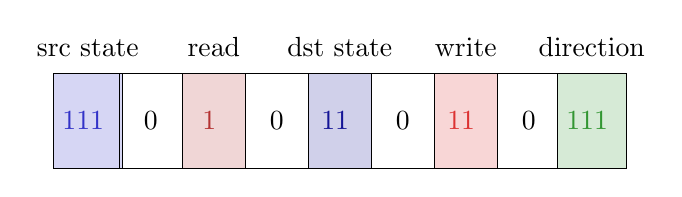
\begin{tikzpicture}
  \tikzset{
    cell/.style={
      draw,
      minimum width=0.8cm,
      minimum height=1.2cm,
      anchor=center
    }
  }
  
  
  % Source state (blue)
  \node[cell, fill=statecolor!20] at (0, 0) {\textcolor{statecolor}{ 111 }};
  \node[above] at (0, 0.7) {src state};
  
  % Separator
  \node[cell] at (0.8, 0) {0};
  
  % Read symbol (red)
  \node[cell, fill=tapesymbolcolor!20] at (1.6, 0) {\textcolor{tapesymbolcolor}{1 }};
  \node[above] at (1.6, 0.7) {read};
  
  % Separator
  \node[cell] at (2.4, 0) {0};
  
  % Destination state (dark blue)
  \node[cell, fill=dststatecolor!20] at (3.2, 0) {\textcolor{dststatecolor}{11 }};
  \node[above] at (3.2, 0.7) {dst state};
  
  % Separator
  \node[cell] at (4.0, 0) {0};
  
  % Write symbol (red)
  \node[cell, fill=writesymbolcolor!20] at (4.8, 0) {\textcolor{writesymbolcolor}{ 11 }};
  \node[above] at (4.8, 0.7) {write};
  
  % Separator
  \node[cell] at (5.6, 0) {0};
  
  % Direction (green)
  \node[cell, fill=directioncolor!20] at (6.4, 0) {\textcolor{directioncolor}{ 111 }};
  \node[above] at (6.4, 0.7) {direction};
\end{tikzpicture}

\section{Step-by-Step UTM Execution}

\subsection*{Step 0: Initial configuration }

\begin{center}
\textbf{ Tape 1 (Encoded TM) }
\end{center}

\begin{center}
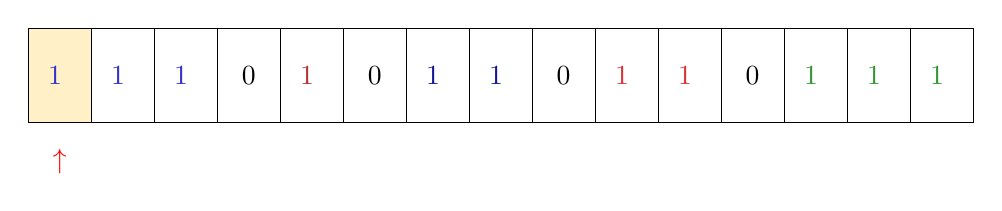
\begin{tikzpicture}
  \tikzset{
    cell/.style={
      draw,
      minimum width=0.8cm,
      minimum height=1.2cm,
      anchor=center,
      fill=white
    },
    highlighted/.style={
      draw,
      minimum width=0.8cm,
      minimum height=1.2cm,
      anchor=center,
      fill=highlightcolor
    },
    decoded/.style={
      font=\footnotesize,
      text=blue
    }
  }
  
  % Draw the tape cells
    \node[highlighted] at (0.0, 0) (cell0) { 
            \textcolor{statecolor}{ 1 }
    };
    \node[below=0.2cm] at (cell0.south) {\color{red}$\uparrow$};
    
    % Add decoded values if available
    \node[cell] at (0.8, 0) (cell1) { 
            \textcolor{statecolor}{ 1 }
    };
    
    % Add decoded values if available
    \node[cell] at (1.6, 0) (cell2) { 
            \textcolor{statecolor}{ 1 }
    };
    
    % Add decoded values if available
    \node[cell] at (2.4000000000000004, 0) (cell3) { 
        0
    };
    
    % Add decoded values if available
    \node[cell] at (3.2, 0) (cell4) { 
            \textcolor{tapesymbolcolor}{ 1 }
    };
    
    % Add decoded values if available
    \node[cell] at (4.0, 0) (cell5) { 
        0
    };
    
    % Add decoded values if available
    \node[cell] at (4.800000000000001, 0) (cell6) { 
            \textcolor{dststatecolor}{ 1 }
    };
    
    % Add decoded values if available
    \node[cell] at (5.6000000000000005, 0) (cell7) { 
            \textcolor{dststatecolor}{ 1 }
    };
    
    % Add decoded values if available
    \node[cell] at (6.4, 0) (cell8) { 
        0
    };
    
    % Add decoded values if available
    \node[cell] at (7.2, 0) (cell9) { 
            \textcolor{writesymbolcolor}{ 1 }
    };
    
    % Add decoded values if available
    \node[cell] at (8.0, 0) (cell10) { 
            \textcolor{writesymbolcolor}{ 1 }
    };
    
    % Add decoded values if available
    \node[cell] at (8.8, 0) (cell11) { 
        0
    };
    
    % Add decoded values if available
    \node[cell] at (9.600000000000001, 0) (cell12) { 
            \textcolor{directioncolor}{ 1 }
    };
    
    % Add decoded values if available
    \node[cell] at (10.4, 0) (cell13) { 
            \textcolor{directioncolor}{ 1 }
    };
    
    % Add decoded values if available
    \node[cell] at (11.200000000000001, 0) (cell14) { 
            \textcolor{directioncolor}{ 1 }
    };
    
    % Add decoded values if available
  
\end{tikzpicture}
\end{center}

\vspace{0.5cm}
\begin{center}
\textbf{ Tape 2 (Input) }
\end{center}

\begin{center}
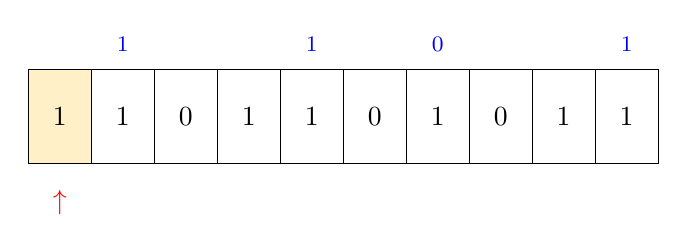
\begin{tikzpicture}
  \tikzset{
    cell/.style={
      draw,
      minimum width=0.8cm,
      minimum height=1.2cm,
      anchor=center,
      fill=white
    },
    highlighted/.style={
      draw,
      minimum width=0.8cm,
      minimum height=1.2cm,
      anchor=center,
      fill=highlightcolor
    },
    decoded/.style={
      font=\footnotesize,
      text=blue
    }
  }
  
  % Draw the tape cells
    \node[highlighted] at (0.0, 0) (cell0) { 
        1
    };
    \node[below=0.2cm] at (cell0.south) {\color{red}$\uparrow$};
    
    % Add decoded values if available
    \node[cell] at (0.8, 0) (cell1) { 
        1
    };
    
    % Add decoded values if available
    \node[decoded, above=0.1cm of cell1] { $1$ };
    \node[cell] at (1.6, 0) (cell2) { 
        0
    };
    
    % Add decoded values if available
    \node[cell] at (2.4000000000000004, 0) (cell3) { 
        1
    };
    
    % Add decoded values if available
    \node[cell] at (3.2, 0) (cell4) { 
        1
    };
    
    % Add decoded values if available
    \node[decoded, above=0.1cm of cell4] { $1$ };
    \node[cell] at (4.0, 0) (cell5) { 
        0
    };
    
    % Add decoded values if available
    \node[cell] at (4.800000000000001, 0) (cell6) { 
        1
    };
    
    % Add decoded values if available
    \node[decoded, above=0.1cm of cell6] { $0$ };
    \node[cell] at (5.6000000000000005, 0) (cell7) { 
        0
    };
    
    % Add decoded values if available
    \node[cell] at (6.4, 0) (cell8) { 
        1
    };
    
    % Add decoded values if available
    \node[cell] at (7.2, 0) (cell9) { 
        1
    };
    
    % Add decoded values if available
    \node[decoded, above=0.1cm of cell9] { $1$ };
  
\end{tikzpicture}
\end{center}

\vspace{0.5cm}
\begin{center}
\textbf{ Tape 3 $(Current State: q_0)$ }
\end{center}

\begin{center}
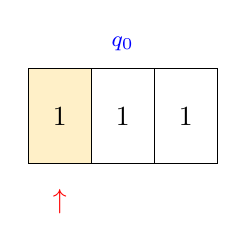
\begin{tikzpicture}
  \tikzset{
    cell/.style={
      draw,
      minimum width=0.8cm,
      minimum height=1.2cm,
      anchor=center,
      fill=white
    },
    highlighted/.style={
      draw,
      minimum width=0.8cm,
      minimum height=1.2cm,
      anchor=center,
      fill=highlightcolor
    },
    decoded/.style={
      font=\footnotesize,
      text=blue
    }
  }
  
  % Draw the tape cells
    \node[highlighted] at (0.0, 0) (cell0) { 
        1
    };
    \node[below=0.2cm] at (cell0.south) {\color{red}$\uparrow$};
    
    % Add decoded values if available
    \node[cell] at (0.8, 0) (cell1) { 
        1
    };
    
    % Add decoded values if available
    \node[decoded, above=0.1cm of cell1] { $q_0$ };
    \node[cell] at (1.6, 0) (cell2) { 
        1
    };
    
    % Add decoded values if available
  
\end{tikzpicture}
\end{center}

\vspace{0.5cm}

\vspace{1cm}
\subsection*{Step 1: $(q_0, 1) \to (q_0, 0, R)$ }

\begin{center}
\textbf{ Tape 1 (Encoded TM) }
\end{center}

\begin{center}
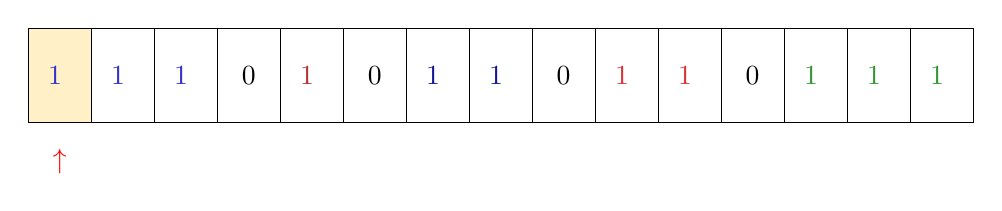
\begin{tikzpicture}
  \tikzset{
    cell/.style={
      draw,
      minimum width=0.8cm,
      minimum height=1.2cm,
      anchor=center,
      fill=white
    },
    highlighted/.style={
      draw,
      minimum width=0.8cm,
      minimum height=1.2cm,
      anchor=center,
      fill=highlightcolor
    },
    decoded/.style={
      font=\footnotesize,
      text=blue
    }
  }
  
  % Draw the tape cells
    \node[highlighted] at (0.0, 0) (cell0) { 
            \textcolor{statecolor}{ 1 }
    };
    \node[below=0.2cm] at (cell0.south) {\color{red}$\uparrow$};
    
    % Add decoded values if available
    \node[cell] at (0.8, 0) (cell1) { 
            \textcolor{statecolor}{ 1 }
    };
    
    % Add decoded values if available
    \node[cell] at (1.6, 0) (cell2) { 
            \textcolor{statecolor}{ 1 }
    };
    
    % Add decoded values if available
    \node[cell] at (2.4000000000000004, 0) (cell3) { 
        0
    };
    
    % Add decoded values if available
    \node[cell] at (3.2, 0) (cell4) { 
            \textcolor{tapesymbolcolor}{ 1 }
    };
    
    % Add decoded values if available
    \node[cell] at (4.0, 0) (cell5) { 
        0
    };
    
    % Add decoded values if available
    \node[cell] at (4.800000000000001, 0) (cell6) { 
            \textcolor{dststatecolor}{ 1 }
    };
    
    % Add decoded values if available
    \node[cell] at (5.6000000000000005, 0) (cell7) { 
            \textcolor{dststatecolor}{ 1 }
    };
    
    % Add decoded values if available
    \node[cell] at (6.4, 0) (cell8) { 
        0
    };
    
    % Add decoded values if available
    \node[cell] at (7.2, 0) (cell9) { 
            \textcolor{writesymbolcolor}{ 1 }
    };
    
    % Add decoded values if available
    \node[cell] at (8.0, 0) (cell10) { 
            \textcolor{writesymbolcolor}{ 1 }
    };
    
    % Add decoded values if available
    \node[cell] at (8.8, 0) (cell11) { 
        0
    };
    
    % Add decoded values if available
    \node[cell] at (9.600000000000001, 0) (cell12) { 
            \textcolor{directioncolor}{ 1 }
    };
    
    % Add decoded values if available
    \node[cell] at (10.4, 0) (cell13) { 
            \textcolor{directioncolor}{ 1 }
    };
    
    % Add decoded values if available
    \node[cell] at (11.200000000000001, 0) (cell14) { 
            \textcolor{directioncolor}{ 1 }
    };
    
    % Add decoded values if available
  
\end{tikzpicture}
\end{center}

\vspace{0.5cm}
\begin{center}
\textbf{ Tape 2 (Input) }
\end{center}

\begin{center}
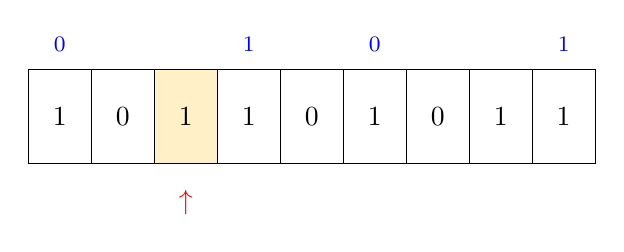
\begin{tikzpicture}
  \tikzset{
    cell/.style={
      draw,
      minimum width=0.8cm,
      minimum height=1.2cm,
      anchor=center,
      fill=white
    },
    highlighted/.style={
      draw,
      minimum width=0.8cm,
      minimum height=1.2cm,
      anchor=center,
      fill=highlightcolor
    },
    decoded/.style={
      font=\footnotesize,
      text=blue
    }
  }
  
  % Draw the tape cells
    \node[cell] at (0.0, 0) (cell0) { 
        1
    };
    
    % Add decoded values if available
    \node[decoded, above=0.1cm of cell0] { $0$ };
    \node[cell] at (0.8, 0) (cell1) { 
        0
    };
    
    % Add decoded values if available
    \node[highlighted] at (1.6, 0) (cell2) { 
        1
    };
    \node[below=0.2cm] at (cell2.south) {\color{red}$\uparrow$};
    
    % Add decoded values if available
    \node[cell] at (2.4000000000000004, 0) (cell3) { 
        1
    };
    
    % Add decoded values if available
    \node[decoded, above=0.1cm of cell3] { $1$ };
    \node[cell] at (3.2, 0) (cell4) { 
        0
    };
    
    % Add decoded values if available
    \node[cell] at (4.0, 0) (cell5) { 
        1
    };
    
    % Add decoded values if available
    \node[decoded, above=0.1cm of cell5] { $0$ };
    \node[cell] at (4.800000000000001, 0) (cell6) { 
        0
    };
    
    % Add decoded values if available
    \node[cell] at (5.6000000000000005, 0) (cell7) { 
        1
    };
    
    % Add decoded values if available
    \node[cell] at (6.4, 0) (cell8) { 
        1
    };
    
    % Add decoded values if available
    \node[decoded, above=0.1cm of cell8] { $1$ };
  
\end{tikzpicture}
\end{center}

\vspace{0.5cm}
\begin{center}
\textbf{ Tape 3 $(Current State: q_0)$ }
\end{center}

\begin{center}
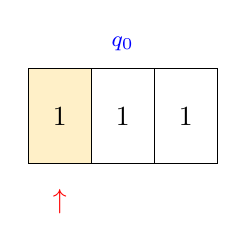
\begin{tikzpicture}
  \tikzset{
    cell/.style={
      draw,
      minimum width=0.8cm,
      minimum height=1.2cm,
      anchor=center,
      fill=white
    },
    highlighted/.style={
      draw,
      minimum width=0.8cm,
      minimum height=1.2cm,
      anchor=center,
      fill=highlightcolor
    },
    decoded/.style={
      font=\footnotesize,
      text=blue
    }
  }
  
  % Draw the tape cells
    \node[highlighted] at (0.0, 0) (cell0) { 
        1
    };
    \node[below=0.2cm] at (cell0.south) {\color{red}$\uparrow$};
    
    % Add decoded values if available
    \node[cell] at (0.8, 0) (cell1) { 
        1
    };
    
    % Add decoded values if available
    \node[decoded, above=0.1cm of cell1] { $q_0$ };
    \node[cell] at (1.6, 0) (cell2) { 
        1
    };
    
    % Add decoded values if available
  
\end{tikzpicture}
\end{center}

\vspace{0.5cm}

\vspace{1cm}
\subsection*{Step 2: $(q_0, 1) \to (q_0, 0, R)$ }

\begin{center}
\textbf{ Tape 1 (Encoded TM) }
\end{center}

\begin{center}
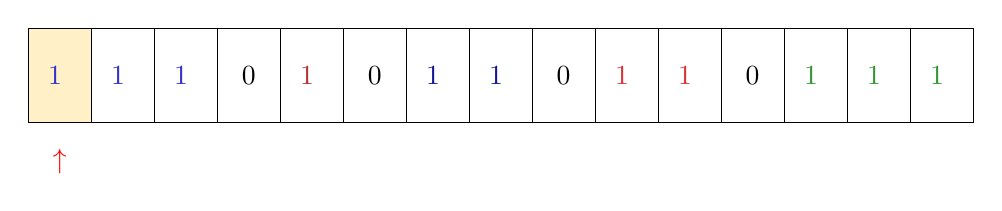
\begin{tikzpicture}
  \tikzset{
    cell/.style={
      draw,
      minimum width=0.8cm,
      minimum height=1.2cm,
      anchor=center,
      fill=white
    },
    highlighted/.style={
      draw,
      minimum width=0.8cm,
      minimum height=1.2cm,
      anchor=center,
      fill=highlightcolor
    },
    decoded/.style={
      font=\footnotesize,
      text=blue
    }
  }
  
  % Draw the tape cells
    \node[highlighted] at (0.0, 0) (cell0) { 
            \textcolor{statecolor}{ 1 }
    };
    \node[below=0.2cm] at (cell0.south) {\color{red}$\uparrow$};
    
    % Add decoded values if available
    \node[cell] at (0.8, 0) (cell1) { 
            \textcolor{statecolor}{ 1 }
    };
    
    % Add decoded values if available
    \node[cell] at (1.6, 0) (cell2) { 
            \textcolor{statecolor}{ 1 }
    };
    
    % Add decoded values if available
    \node[cell] at (2.4000000000000004, 0) (cell3) { 
        0
    };
    
    % Add decoded values if available
    \node[cell] at (3.2, 0) (cell4) { 
            \textcolor{tapesymbolcolor}{ 1 }
    };
    
    % Add decoded values if available
    \node[cell] at (4.0, 0) (cell5) { 
        0
    };
    
    % Add decoded values if available
    \node[cell] at (4.800000000000001, 0) (cell6) { 
            \textcolor{dststatecolor}{ 1 }
    };
    
    % Add decoded values if available
    \node[cell] at (5.6000000000000005, 0) (cell7) { 
            \textcolor{dststatecolor}{ 1 }
    };
    
    % Add decoded values if available
    \node[cell] at (6.4, 0) (cell8) { 
        0
    };
    
    % Add decoded values if available
    \node[cell] at (7.2, 0) (cell9) { 
            \textcolor{writesymbolcolor}{ 1 }
    };
    
    % Add decoded values if available
    \node[cell] at (8.0, 0) (cell10) { 
            \textcolor{writesymbolcolor}{ 1 }
    };
    
    % Add decoded values if available
    \node[cell] at (8.8, 0) (cell11) { 
        0
    };
    
    % Add decoded values if available
    \node[cell] at (9.600000000000001, 0) (cell12) { 
            \textcolor{directioncolor}{ 1 }
    };
    
    % Add decoded values if available
    \node[cell] at (10.4, 0) (cell13) { 
            \textcolor{directioncolor}{ 1 }
    };
    
    % Add decoded values if available
    \node[cell] at (11.200000000000001, 0) (cell14) { 
            \textcolor{directioncolor}{ 1 }
    };
    
    % Add decoded values if available
  
\end{tikzpicture}
\end{center}

\vspace{0.5cm}
\begin{center}
\textbf{ Tape 2 (Input) }
\end{center}

\begin{center}
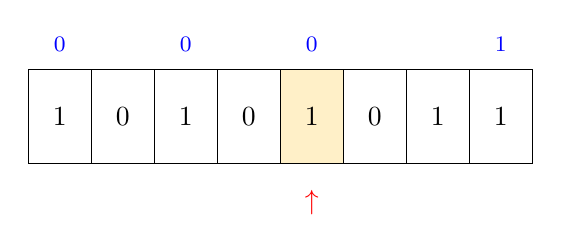
\begin{tikzpicture}
  \tikzset{
    cell/.style={
      draw,
      minimum width=0.8cm,
      minimum height=1.2cm,
      anchor=center,
      fill=white
    },
    highlighted/.style={
      draw,
      minimum width=0.8cm,
      minimum height=1.2cm,
      anchor=center,
      fill=highlightcolor
    },
    decoded/.style={
      font=\footnotesize,
      text=blue
    }
  }
  
  % Draw the tape cells
    \node[cell] at (0.0, 0) (cell0) { 
        1
    };
    
    % Add decoded values if available
    \node[decoded, above=0.1cm of cell0] { $0$ };
    \node[cell] at (0.8, 0) (cell1) { 
        0
    };
    
    % Add decoded values if available
    \node[cell] at (1.6, 0) (cell2) { 
        1
    };
    
    % Add decoded values if available
    \node[decoded, above=0.1cm of cell2] { $0$ };
    \node[cell] at (2.4000000000000004, 0) (cell3) { 
        0
    };
    
    % Add decoded values if available
    \node[highlighted] at (3.2, 0) (cell4) { 
        1
    };
    \node[below=0.2cm] at (cell4.south) {\color{red}$\uparrow$};
    
    % Add decoded values if available
    \node[decoded, above=0.1cm of cell4] { $0$ };
    \node[cell] at (4.0, 0) (cell5) { 
        0
    };
    
    % Add decoded values if available
    \node[cell] at (4.800000000000001, 0) (cell6) { 
        1
    };
    
    % Add decoded values if available
    \node[cell] at (5.6000000000000005, 0) (cell7) { 
        1
    };
    
    % Add decoded values if available
    \node[decoded, above=0.1cm of cell7] { $1$ };
  
\end{tikzpicture}
\end{center}

\vspace{0.5cm}
\begin{center}
\textbf{ Tape 3 $(Current State: q_0)$ }
\end{center}

\begin{center}
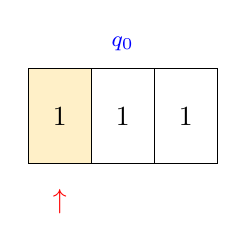
\begin{tikzpicture}
  \tikzset{
    cell/.style={
      draw,
      minimum width=0.8cm,
      minimum height=1.2cm,
      anchor=center,
      fill=white
    },
    highlighted/.style={
      draw,
      minimum width=0.8cm,
      minimum height=1.2cm,
      anchor=center,
      fill=highlightcolor
    },
    decoded/.style={
      font=\footnotesize,
      text=blue
    }
  }
  
  % Draw the tape cells
    \node[highlighted] at (0.0, 0) (cell0) { 
        1
    };
    \node[below=0.2cm] at (cell0.south) {\color{red}$\uparrow$};
    
    % Add decoded values if available
    \node[cell] at (0.8, 0) (cell1) { 
        1
    };
    
    % Add decoded values if available
    \node[decoded, above=0.1cm of cell1] { $q_0$ };
    \node[cell] at (1.6, 0) (cell2) { 
        1
    };
    
    % Add decoded values if available
  
\end{tikzpicture}
\end{center}

\vspace{0.5cm}

\vspace{1cm}
\subsection*{Step 3: $(q_0, 0) \to (q_a, 1, N)$ }

\begin{center}
\textbf{ Tape 1 (Encoded TM) }
\end{center}

\begin{center}
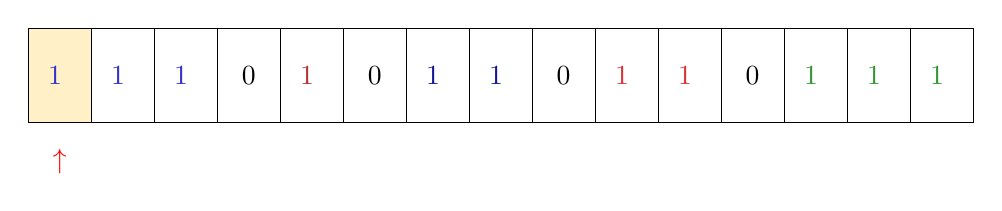
\begin{tikzpicture}
  \tikzset{
    cell/.style={
      draw,
      minimum width=0.8cm,
      minimum height=1.2cm,
      anchor=center,
      fill=white
    },
    highlighted/.style={
      draw,
      minimum width=0.8cm,
      minimum height=1.2cm,
      anchor=center,
      fill=highlightcolor
    },
    decoded/.style={
      font=\footnotesize,
      text=blue
    }
  }
  
  % Draw the tape cells
    \node[highlighted] at (0.0, 0) (cell0) { 
            \textcolor{statecolor}{ 1 }
    };
    \node[below=0.2cm] at (cell0.south) {\color{red}$\uparrow$};
    
    % Add decoded values if available
    \node[cell] at (0.8, 0) (cell1) { 
            \textcolor{statecolor}{ 1 }
    };
    
    % Add decoded values if available
    \node[cell] at (1.6, 0) (cell2) { 
            \textcolor{statecolor}{ 1 }
    };
    
    % Add decoded values if available
    \node[cell] at (2.4000000000000004, 0) (cell3) { 
        0
    };
    
    % Add decoded values if available
    \node[cell] at (3.2, 0) (cell4) { 
            \textcolor{tapesymbolcolor}{ 1 }
    };
    
    % Add decoded values if available
    \node[cell] at (4.0, 0) (cell5) { 
        0
    };
    
    % Add decoded values if available
    \node[cell] at (4.800000000000001, 0) (cell6) { 
            \textcolor{dststatecolor}{ 1 }
    };
    
    % Add decoded values if available
    \node[cell] at (5.6000000000000005, 0) (cell7) { 
            \textcolor{dststatecolor}{ 1 }
    };
    
    % Add decoded values if available
    \node[cell] at (6.4, 0) (cell8) { 
        0
    };
    
    % Add decoded values if available
    \node[cell] at (7.2, 0) (cell9) { 
            \textcolor{writesymbolcolor}{ 1 }
    };
    
    % Add decoded values if available
    \node[cell] at (8.0, 0) (cell10) { 
            \textcolor{writesymbolcolor}{ 1 }
    };
    
    % Add decoded values if available
    \node[cell] at (8.8, 0) (cell11) { 
        0
    };
    
    % Add decoded values if available
    \node[cell] at (9.600000000000001, 0) (cell12) { 
            \textcolor{directioncolor}{ 1 }
    };
    
    % Add decoded values if available
    \node[cell] at (10.4, 0) (cell13) { 
            \textcolor{directioncolor}{ 1 }
    };
    
    % Add decoded values if available
    \node[cell] at (11.200000000000001, 0) (cell14) { 
            \textcolor{directioncolor}{ 1 }
    };
    
    % Add decoded values if available
  
\end{tikzpicture}
\end{center}

\vspace{0.5cm}
\begin{center}
\textbf{ Tape 2 (Input) }
\end{center}

\begin{center}
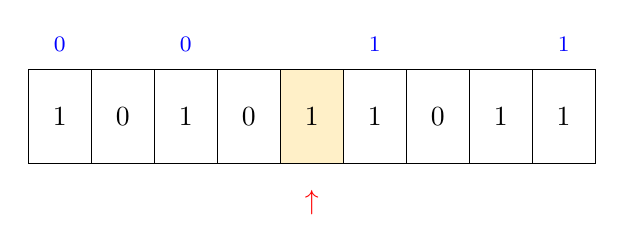
\begin{tikzpicture}
  \tikzset{
    cell/.style={
      draw,
      minimum width=0.8cm,
      minimum height=1.2cm,
      anchor=center,
      fill=white
    },
    highlighted/.style={
      draw,
      minimum width=0.8cm,
      minimum height=1.2cm,
      anchor=center,
      fill=highlightcolor
    },
    decoded/.style={
      font=\footnotesize,
      text=blue
    }
  }
  
  % Draw the tape cells
    \node[cell] at (0.0, 0) (cell0) { 
        1
    };
    
    % Add decoded values if available
    \node[decoded, above=0.1cm of cell0] { $0$ };
    \node[cell] at (0.8, 0) (cell1) { 
        0
    };
    
    % Add decoded values if available
    \node[cell] at (1.6, 0) (cell2) { 
        1
    };
    
    % Add decoded values if available
    \node[decoded, above=0.1cm of cell2] { $0$ };
    \node[cell] at (2.4000000000000004, 0) (cell3) { 
        0
    };
    
    % Add decoded values if available
    \node[highlighted] at (3.2, 0) (cell4) { 
        1
    };
    \node[below=0.2cm] at (cell4.south) {\color{red}$\uparrow$};
    
    % Add decoded values if available
    \node[cell] at (4.0, 0) (cell5) { 
        1
    };
    
    % Add decoded values if available
    \node[decoded, above=0.1cm of cell5] { $1$ };
    \node[cell] at (4.800000000000001, 0) (cell6) { 
        0
    };
    
    % Add decoded values if available
    \node[cell] at (5.6000000000000005, 0) (cell7) { 
        1
    };
    
    % Add decoded values if available
    \node[cell] at (6.4, 0) (cell8) { 
        1
    };
    
    % Add decoded values if available
    \node[decoded, above=0.1cm of cell8] { $1$ };
  
\end{tikzpicture}
\end{center}

\vspace{0.5cm}
\begin{center}
\textbf{ Tape 3 $(Current State: q_a)$ }
\end{center}

\begin{center}
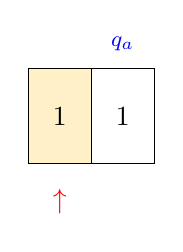
\begin{tikzpicture}
  \tikzset{
    cell/.style={
      draw,
      minimum width=0.8cm,
      minimum height=1.2cm,
      anchor=center,
      fill=white
    },
    highlighted/.style={
      draw,
      minimum width=0.8cm,
      minimum height=1.2cm,
      anchor=center,
      fill=highlightcolor
    },
    decoded/.style={
      font=\footnotesize,
      text=blue
    }
  }
  
  % Draw the tape cells
    \node[highlighted] at (0.0, 0) (cell0) { 
        1
    };
    \node[below=0.2cm] at (cell0.south) {\color{red}$\uparrow$};
    
    % Add decoded values if available
    \node[cell] at (0.8, 0) (cell1) { 
        1
    };
    
    % Add decoded values if available
    \node[decoded, above=0.1cm of cell1] { $q_a$ };
  
\end{tikzpicture}
\end{center}

\vspace{0.5cm}

\vspace{1cm}
\subsection*{Step 4: No matching transition found: reject }

\begin{center}
\textbf{ Tape 1 (Encoded TM) }
\end{center}

\begin{center}
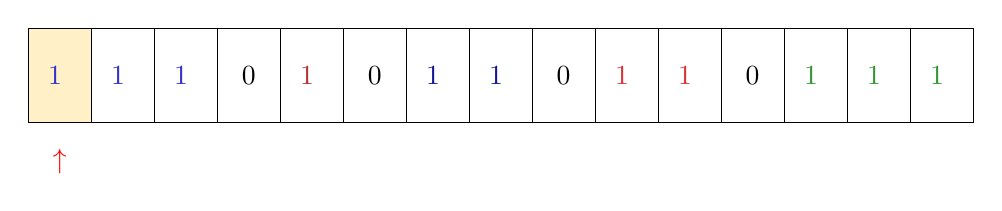
\begin{tikzpicture}
  \tikzset{
    cell/.style={
      draw,
      minimum width=0.8cm,
      minimum height=1.2cm,
      anchor=center,
      fill=white
    },
    highlighted/.style={
      draw,
      minimum width=0.8cm,
      minimum height=1.2cm,
      anchor=center,
      fill=highlightcolor
    },
    decoded/.style={
      font=\footnotesize,
      text=blue
    }
  }
  
  % Draw the tape cells
    \node[highlighted] at (0.0, 0) (cell0) { 
            \textcolor{statecolor}{ 1 }
    };
    \node[below=0.2cm] at (cell0.south) {\color{red}$\uparrow$};
    
    % Add decoded values if available
    \node[cell] at (0.8, 0) (cell1) { 
            \textcolor{statecolor}{ 1 }
    };
    
    % Add decoded values if available
    \node[cell] at (1.6, 0) (cell2) { 
            \textcolor{statecolor}{ 1 }
    };
    
    % Add decoded values if available
    \node[cell] at (2.4000000000000004, 0) (cell3) { 
        0
    };
    
    % Add decoded values if available
    \node[cell] at (3.2, 0) (cell4) { 
            \textcolor{tapesymbolcolor}{ 1 }
    };
    
    % Add decoded values if available
    \node[cell] at (4.0, 0) (cell5) { 
        0
    };
    
    % Add decoded values if available
    \node[cell] at (4.800000000000001, 0) (cell6) { 
            \textcolor{dststatecolor}{ 1 }
    };
    
    % Add decoded values if available
    \node[cell] at (5.6000000000000005, 0) (cell7) { 
            \textcolor{dststatecolor}{ 1 }
    };
    
    % Add decoded values if available
    \node[cell] at (6.4, 0) (cell8) { 
        0
    };
    
    % Add decoded values if available
    \node[cell] at (7.2, 0) (cell9) { 
            \textcolor{writesymbolcolor}{ 1 }
    };
    
    % Add decoded values if available
    \node[cell] at (8.0, 0) (cell10) { 
            \textcolor{writesymbolcolor}{ 1 }
    };
    
    % Add decoded values if available
    \node[cell] at (8.8, 0) (cell11) { 
        0
    };
    
    % Add decoded values if available
    \node[cell] at (9.600000000000001, 0) (cell12) { 
            \textcolor{directioncolor}{ 1 }
    };
    
    % Add decoded values if available
    \node[cell] at (10.4, 0) (cell13) { 
            \textcolor{directioncolor}{ 1 }
    };
    
    % Add decoded values if available
    \node[cell] at (11.200000000000001, 0) (cell14) { 
            \textcolor{directioncolor}{ 1 }
    };
    
    % Add decoded values if available
  
\end{tikzpicture}
\end{center}

\vspace{0.5cm}
\begin{center}
\textbf{ Tape 2 (Input) }
\end{center}

\begin{center}
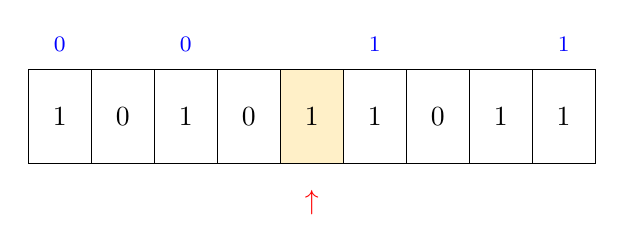
\begin{tikzpicture}
  \tikzset{
    cell/.style={
      draw,
      minimum width=0.8cm,
      minimum height=1.2cm,
      anchor=center,
      fill=white
    },
    highlighted/.style={
      draw,
      minimum width=0.8cm,
      minimum height=1.2cm,
      anchor=center,
      fill=highlightcolor
    },
    decoded/.style={
      font=\footnotesize,
      text=blue
    }
  }
  
  % Draw the tape cells
    \node[cell] at (0.0, 0) (cell0) { 
        1
    };
    
    % Add decoded values if available
    \node[decoded, above=0.1cm of cell0] { $0$ };
    \node[cell] at (0.8, 0) (cell1) { 
        0
    };
    
    % Add decoded values if available
    \node[cell] at (1.6, 0) (cell2) { 
        1
    };
    
    % Add decoded values if available
    \node[decoded, above=0.1cm of cell2] { $0$ };
    \node[cell] at (2.4000000000000004, 0) (cell3) { 
        0
    };
    
    % Add decoded values if available
    \node[highlighted] at (3.2, 0) (cell4) { 
        1
    };
    \node[below=0.2cm] at (cell4.south) {\color{red}$\uparrow$};
    
    % Add decoded values if available
    \node[cell] at (4.0, 0) (cell5) { 
        1
    };
    
    % Add decoded values if available
    \node[decoded, above=0.1cm of cell5] { $1$ };
    \node[cell] at (4.800000000000001, 0) (cell6) { 
        0
    };
    
    % Add decoded values if available
    \node[cell] at (5.6000000000000005, 0) (cell7) { 
        1
    };
    
    % Add decoded values if available
    \node[cell] at (6.4, 0) (cell8) { 
        1
    };
    
    % Add decoded values if available
    \node[decoded, above=0.1cm of cell8] { $1$ };
  
\end{tikzpicture}
\end{center}

\vspace{0.5cm}
\begin{center}
\textbf{ Tape 3 $(Current State: q_a)$ }
\end{center}

\begin{center}
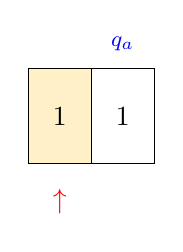
\begin{tikzpicture}
  \tikzset{
    cell/.style={
      draw,
      minimum width=0.8cm,
      minimum height=1.2cm,
      anchor=center,
      fill=white
    },
    highlighted/.style={
      draw,
      minimum width=0.8cm,
      minimum height=1.2cm,
      anchor=center,
      fill=highlightcolor
    },
    decoded/.style={
      font=\footnotesize,
      text=blue
    }
  }
  
  % Draw the tape cells
    \node[highlighted] at (0.0, 0) (cell0) { 
        1
    };
    \node[below=0.2cm] at (cell0.south) {\color{red}$\uparrow$};
    
    % Add decoded values if available
    \node[cell] at (0.8, 0) (cell1) { 
        1
    };
    
    % Add decoded values if available
    \node[decoded, above=0.1cm of cell1] { $q_a$ };
  
\end{tikzpicture}
\end{center}

\vspace{0.5cm}

\vspace{1cm}

\end{document}